\documentclass[12pt,letterpaper]{article}
\usepackage{graphicx}
\usepackage{geometry}
\usepackage{setspace}
\usepackage{anyfontsize}
\usepackage{parskip}
\usepackage{indentfirst}
\usepackage{amsmath}
\usepackage{listings}
\usepackage{color}
\usepackage{textcomp}
\usepackage{float}
\usepackage[utf8]{inputenc}
\usepackage[backend=biber,style=ieee,natbib=true]{biblatex}
\usepackage{subcaption}
\usepackage{hyperref}
\usepackage{enumitem}
\usepackage{csvsimple}

\geometry{letterpaper, portrait, margin=1in}
\doublespace
\title{Modelling Drugs and JUULs on PAR}
\author{Team \#11745}
\graphicspath{{./imgs/}}
\addbibresource{m3c.bib}

\hypersetup{
	colorlinks=true,
	linkcolor=black,
	filecolor=magenta,
	urlcolor=cyan,
	citecolor=blue,
}

\definecolor{codegreen}{rgb}{0,0.6,0}
\definecolor{codegray}{rgb}{0.5,0.5,0.5}
\definecolor{codepurple}{rgb}{0.58,0,0.82}
\definecolor{backcolor}{rgb}{0.95,0.95,0.95}

\lstdefinestyle{scheme}{
    backgroundcolor=\color{backcolor},
    commentstyle=\color{codegray},
    keywordstyle=\color{blue},
    numberstyle=\tiny\color{codegray},
    stringstyle=\color{red},
    basicstyle=\footnotesize\ttfamily,
    breakatwhitespace=false,
    breaklines=true,
    captionpos=t,
    keepspaces=true,
    numbers=left,
    numbersep=5pt,
    showspaces=false,
    showstringspaces=false,
    showtabs=false,
    tabsize=2
}

\lstset{style=scheme}

\usepackage{fancyhdr}
\pagestyle{fancy}
\fancyhf{}
\chead{Team \#11745}
\cfoot{\thepage}

\begin{document}
\parindent=0.5in

\maketitle

\subsection*{Executive Summary}
\begin{singlespace}
\begin{small}
In the United States, the recreational use of illicit substances has grown an incredible amount in recent years. In more recent years, the prevalence of vaping in the form of using JUULs has increased to the point where one cannot walk down a hall and not see a JUUL in the hands of someone. However, there are many other substances that are also used and abused in high school. JUUL usage has introduced a young population to nicotine, which has caused many in this population to become addicted.

Our models show that JUUL usage will probably grow which will cause a shrinkage in cigarette usage. This leads to a decrease in mortality related to nicotine intake. We also applied our model to many different drugs and found that as the physical and psychological effects of a given substance increased, the less likely it would be to spread. We used a “potential - addicted - recovered” (PAR) model where some of the recovered are fed back into the potential because some people may stop using a drug and then relapse again. We adjusted the coefficients in this model in order to achieve our desired effects based on the previously determined data from previous years which we tested on a few substances that we knew we would not be testing. We then used this model to attempt to predict the values for the substances we knew we would be testing and found our model to be incredibly accurate. We used the Dunbar tiers based on the Dunbar number to find the value for the number of close friends a given person has, and then found the percent of one’s close friends that would use a given drug. This allowed for the external social pressure of social settings to be applied to the model. 

Furthermore, we also created a metric of how bad a given drug is, where marijuana is the least dangerous in terms of qualitative data and opioids are the most dangerous. As we calculated our PAR model, we added the estimated daily national cost of jail, medical costs, lost commerce, and lost taxes. While our models are quite complicated, they were fairly accurate when compared to the data for a given class in the future if given the data from that class was collected before hand. This allowed us to be fairly confident in the future predictions that the model was producing.
\end{small}
\end{singlespace}

\newpage
\tableofcontents

\newpage
\section{Global Identifications}
\subsection{Global Assumptions}
\begin{itemize}
  \item Sources of information, data, and models in this investigation pertain only to the United States population.
  \item Differences in factors between genders will be ignored because the input data is gender agnostic and any gender-based lurking variables will equalize within the sample size of data and simulations.
  \item One year is equal to 365 days.
  \item A high school is a closed-system.
  \item The entire US population has an equal tolerance level to all drugs.
  \item Our model does not take death of any kind into account.
\end{itemize}

\subsection{Global Definitions}
\begin{itemize}
\item “Substance” is any kind of drug, which is something that has psychological effects on a person.
\item “Use” is the intake of a drug either through smoking, vaporizing, injecting, nasal inhalation of a substance or ingestion of pills of a given substance orally.
\end{itemize}

\section{Darth Vapor}
\subsection{Local Assumptions}
\begin{itemize}
  \item One cigarette contains 12 mg of nicotine \citep{matthews_how_2017}
  \item The rate of absorption of nicotine from one cigarette is 1 mg per cigarette because there is loss from the combustion of the cigarette and filtering. Our unit of 1 cigarette of nicotine indicates the rate of nicotine intake, 1 mg per cigarette, and not nicotine content, 12 mg per cigarette. \citep[501]{benowitz_daily_1984}
  \item One cigarette is worth 10 puffs. \citep{noauthor_e-cigarette_2014}
  \item One pack of cigarettes costs \$5 and contains 20 cigarettes.
  \item Our model assumes JUULs as the unit of vape consumption and encapsulates e-cigarettes for this model.
  \item The JUUL device kit costs \$35 for the device and charger and is the base cost of entry for JUUL. \citep{noauthor_juul_nodate}
  \item Four JUUL pods cost \$16. \citep{noauthor_buy_nodate}
  \item A JUUL pod has negligible nicotine waste becasue there is no combustion or filter.
  \item One JUUL pod 41 mg or approximately 40 cigarettes worth of nicotine absorption. \citep{noauthor_juulpods_nodate}
  \item Socio-economic factors do not affect substance use to a significant degree,\citep{simon_socioeconomic_2018} it was more based off of advertising and exposure.\citep{redonnet_tobacco_2012} However, this varied greatly such that it could not reliable added to the model.
  \item It is assumed that 14\% of U.S. adults over the age of 18 currently smoke cigarettes.\citep{cdc_current_2019}
\end{itemize}

\subsection{Restatement of Problem}
We were asked to create a model to predict the spread of nicotine usage due to vaping over the next 10 years, and then asked to compare that to cigarettes.

\subsection{Solution and Results}
The problem statement asks for us to compare the spread of nicotine intake due to vaping against the spread of nicotine use due to the smoking of cigarettes. To do this we used a modified version of the “susceptible - infected - recovered” (SIR) model where the susceptible people are the people who have not ingested any nicotine from vaping or cigarettes in one month, the infected people are those that have ingested nicotine from vaping or cigarettes in the last month, and the recovered people are the people who have not done nicotine in the future. The model will be referred to as PAR. We modified this model slightly as we feed some of the recovered people back into the infected category as the people who try to quit smoking but eventually relapse back into it. We chose to use this model because we noticed an upward trend in the use of E-Cigarettes (see Figure \ref{fig:cigusage}). These all show a trend which we thought could be well represented by a PAR model. For smoking, the model would be called PSR, referring to active smokers as the infected population. We created the following model to model the usage of vaping for nicotine, as well as cigarettes.

\begin{figure}[H]
  \centering
  \begin{subfigure}[t]{.3\linewidth}
  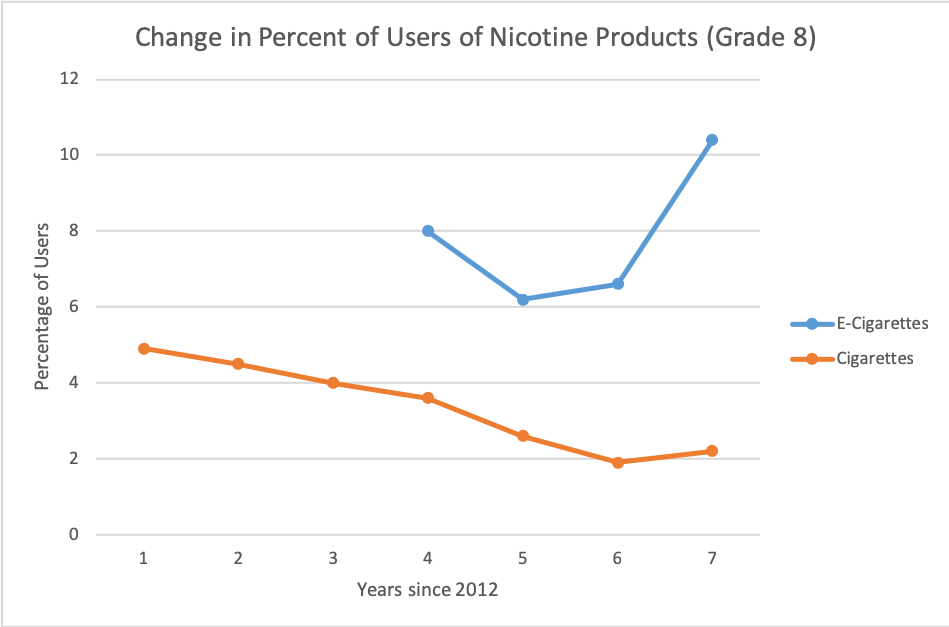
\includegraphics[width=\linewidth]{percentUsers8}
  \end{subfigure}
  \begin{subfigure}[t]{.3\linewidth}
  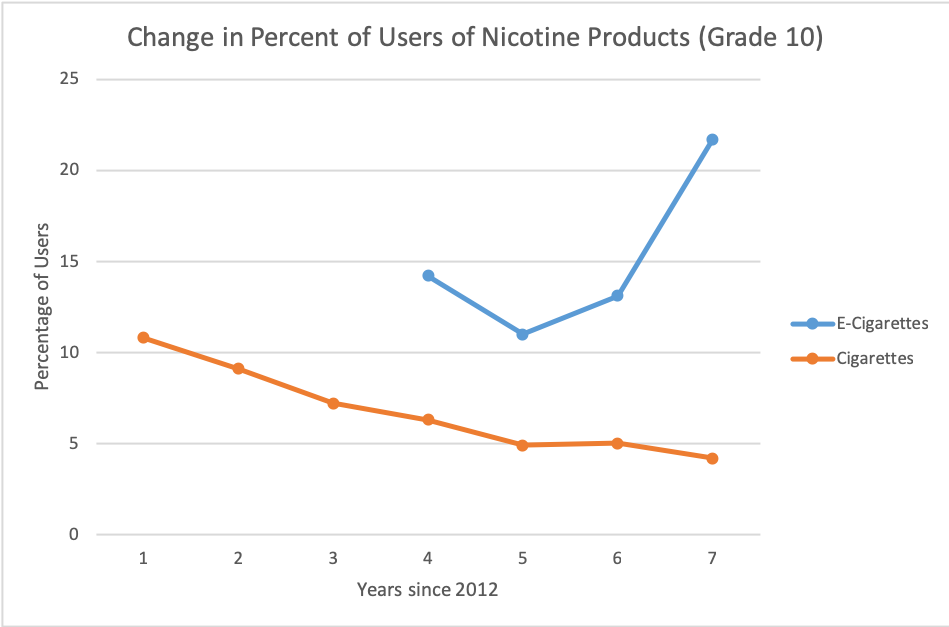
\includegraphics[width=\linewidth]{percentUsers10}
  \end{subfigure}
  \begin{subfigure}[t]{.3\linewidth}
  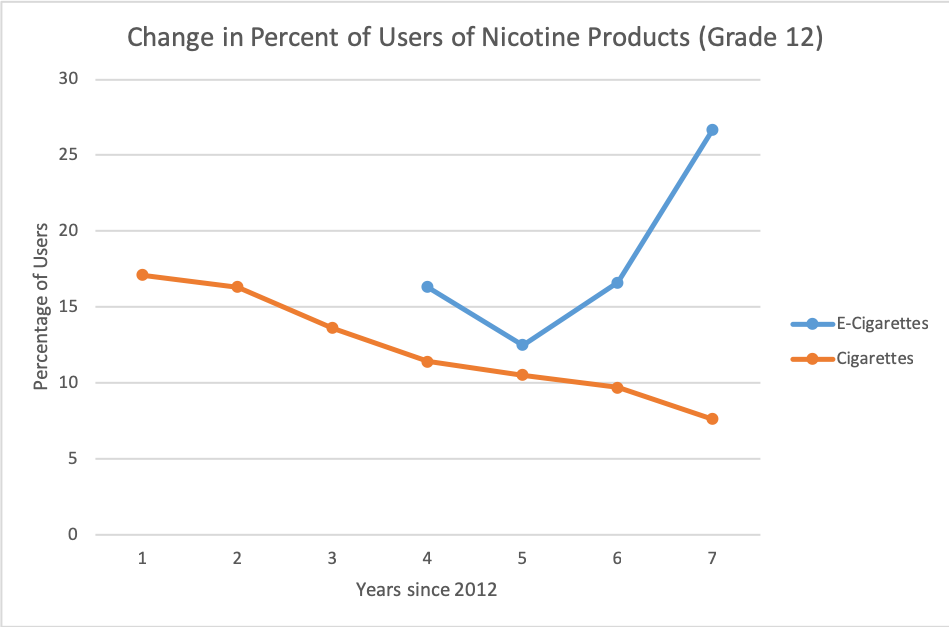
\includegraphics[width=\linewidth]{percentUsers12}
  \end{subfigure}
  
  \begin{subfigure}[t]{.4\linewidth}
  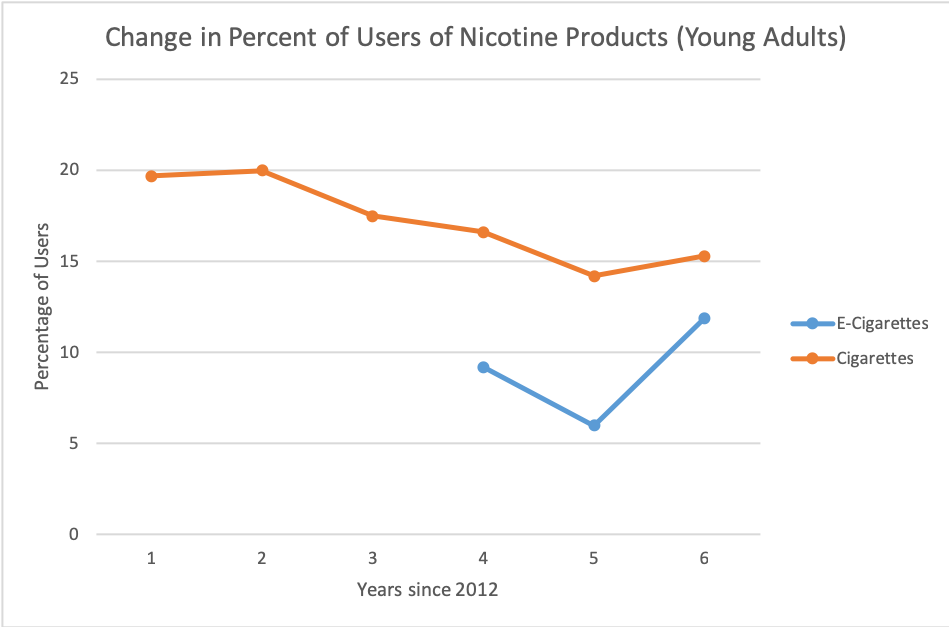
\includegraphics[width=\linewidth]{percentUsersYA}
  \end{subfigure}
  \begin{subfigure}[t]{.4\linewidth}
  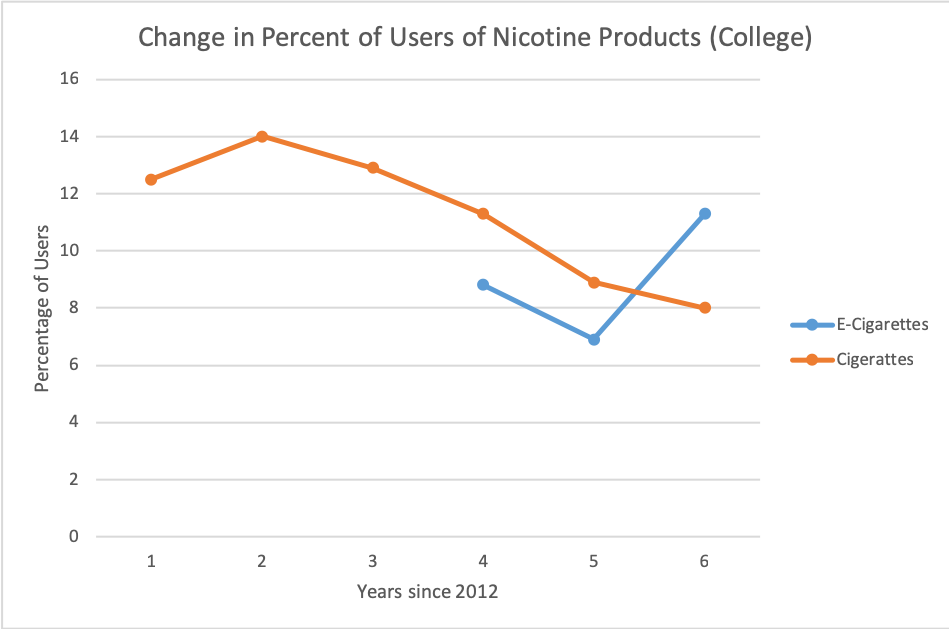
\includegraphics[width=\linewidth]{percentUsersCo}
  \end{subfigure}
  \caption{Vape vs. Cigarette Usage by Age Group \citep{noauthor_college-age_2018}}
  \label{fig:cigusage}
\end{figure}

These models show that vaping usage will increase to a point and then plateau, and that the usage of cigarettes would decrease over the next 10 years. We also conducted a cost analysis of JUULs vs. Cigarettes which shows when JUULs become more efficient to use than cigarettes. Section \ref{sec:cost} is our cost analysis of JUULs vs. Cigarettes.

\begin{figure}[H]
  \centering
  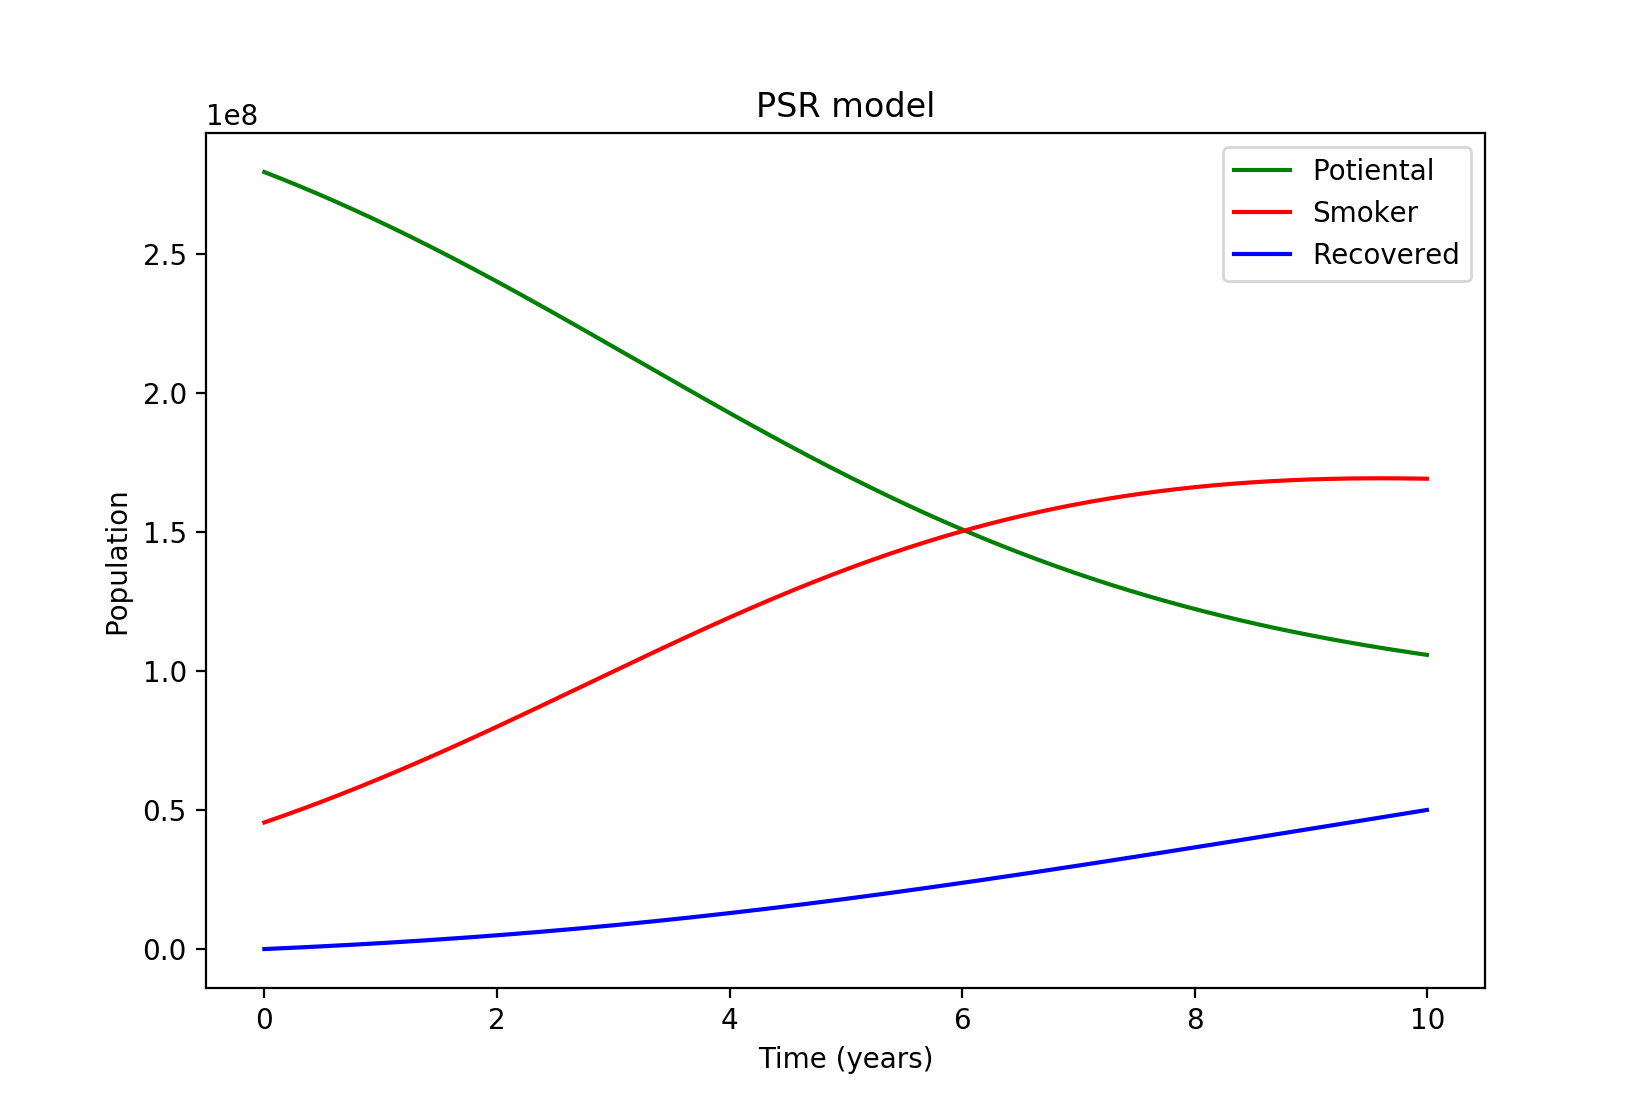
\includegraphics[width=.8\linewidth]{PSR}
  \caption{PSR for the total US population}
  \label{fig:PSR}
\end{figure}

\begin{singlespace}
\begin{small}
\begin{equation}
\label{eq:1}
\begin{aligned}
\frac{dP}{dt} &= -\beta \frac{PS}{N} + \alpha ( 1 - \epsilon )S \\
\frac{dS}{dt} &= \beta \frac{PS}{N} - \alpha S \\
\frac{dR}{dt} &= \alpha \epsilon S
\end{aligned}
\end{equation}
\begin{itemize}[label=]
  \item $S$ = Smokers
  \item $P$ = Potential addicts
  \item $\beta$ = Rate of transmission
  \item $\alpha$ = Rate of recovery
  \item $1 - \epsilon$ = Rate of relapse
  \item $R$ = Smoking quitters
  \item $N$ = Total population
\end{itemize}
\end{small}
\end{singlespace}

\subsection{Cost Analysis of JUULs vs. Cigarettes}
\label{sec:cost}
To determine which form of nicotine intake is more cost effective over time, two linear equations were constructed for each, where $y$ is the total cost and $x$ is each additional cigarette (synonymous with each additional intake of 1 mg of nicotine).

\begin{figure}[H]
  \centering
  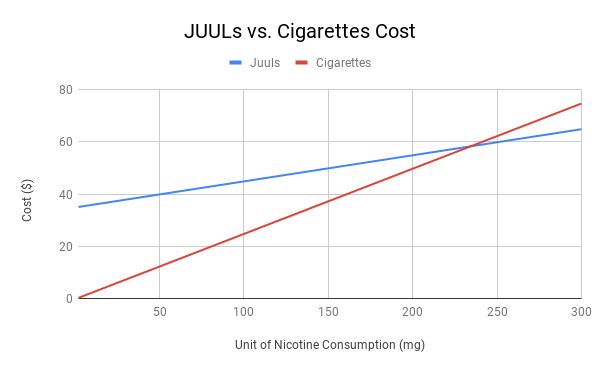
\includegraphics[width=.7\linewidth]{JUULs-vs-Cigarettes-Cost}
  \caption{JUULs vs. Cigarettes Cost}
  \label{fig:cigcosts}
\end{figure}

\paragraph{JUUL}
\begin{equation}
\label{eq:juul}
y = \frac{16}{160} x + 35
\end{equation}
  \begin{itemize}
  	\item Slope $\frac{16}{160}$ = cost per each additional cigarette, aka each additional cigarette worth of nicotine intake (1 mg).
  	  \subitem 16 = the cost of four JUUL pods; JUUL pods are sold in packs of four for \$15.99.
  	  \subitem 160 = the number of milligrams of nicotine in 4 pods (approximately 40 milligrams of nicotine per pod).
  	\item 35 = cost of device kit (\$34.99), which includes a JUUL device and charger.
  \end{itemize}
\paragraph{Cigarette}
\begin{equation}
\label{eq:cig}
y = \frac{5}{20} x
\end{equation}
  \begin{itemize}
    \item Slope $\frac{5}{20}$ = Cost per each additional cigarette, aka each additional cigarette’s worth of nicotine intake (1 mg).
      \subitem 5 = simplified cost per pack of cigarette.
      \subitem 20 = number of milligrams of nicotine absorbed per pack.
  \end{itemize}

Equations \ref{eq:juul} and \ref{eq:cig} intersect at 233 mg of nicotine and at \$58. This shows that when you plan to consume more than 233 mg of nicotine, it is more efficient to buy a JUUL and JUUL pods instead of cigarettes. These show that less money will be spent in the nicotine industry, but specifically in the vaping industry, in the long run. This will cause cigarette production to decrease because people will be switching to vaping, thus decreasing number of people smoking cigarettes, but these ramifications will be after the 10 year period we have been asked to evaluate.

Given the differential equation in Equation \ref{eq:1}, $\beta \frac{PS}{n}$ is the number of people that get addicted since it can be assumed that the number of people that become addicted increases as there are more people around, $P$. $\alpha S$ is the number of people that quit the drug. The $\epsilon$ is the percentage of people that stay recovered. That's the reason that the change in quitters is $\alpha\epsilon S$ and there is $1-\epsilon$ for the potential addicts. The $\epsilon$ also represents the amount of people that can relapse back into addiction which is why they were fed into the potential pool. This ability to feed people back into the susceptible population is what differentiates our model from the traditional SIR model. A high $\epsilon$ means that people try to quit multiple times. A high $\alpha$ represents a high number of people that quit. If there is a drug that has a high $\epsilon$ and $\alpha$ then it is typically a recreational drug. A drug with a high $\beta$ and low $\alpha$ is a highly addicting drug.  

\subsection{Strengths and Weaknesses}
\paragraph{Strengths}
\begin{itemize}
\item Complexity: Despite its difficulty to use, the complexity of the model makes it to produce more accurate extrapolations that are more likely to follow the shown trends of the data.
\item Accuracy: The model is able to be more accurate due to its ability to predict values from already known data and using it to create future predictions that model current trends that allow for a more wide variety of factors to be accounted for.
\end{itemize}

\paragraph{Weaknesses}
\begin{itemize}
\item Model Variables: The values are not empirically supported due to the fact that these values are not available on their own and may not be necessarily true or perfectly accurate. However, based on the data shown in \ref{fig:cigusage}, the values were able to be approximated in order to create the model. 
\item Complexity: The complexity of our model makes it more difficult to use and also means that any changes to it may make it more susceptible to not working if any value is incorrect, inaccurate, or outside the expected inputs such that a vastly inaccurate output could be produced.
\item Bias: Response bias plays a large role in our data, so if response bias leads to significant data skew, our model and data is thrown off completely.
\end{itemize}

\section{Above or Under the Influence?}

\subsection{Local Assumptions}

\begin{itemize}
  \item The proportion of deaths caused by opium overdose is negligible.
  \item The gateway nature of marijuana doesn’t need to be identified as its own variable because the reasons (behind why marijuana leads to opioid usage) can be woven into the other variables.
\end{itemize}

\subsection{Restatement of Problem}
We were asked to create a model that estimates the likelihood that an individual will use a given substance, while taking into account many different factors. After we find a model for all the different substances, we were asked to apply it to a class of 300 high school seniors and estimate how many of them will use a given substance, and the substances we were asked to look at were nicotine, marijuana, alcohol, and un-prescribed opioids.

\paragraph{Variables}
\begin{itemize}[label=]
  \item $P$ = Initial potential addicts
  \item $A$ = Initial Addicts, baseline drug addition of health affects and genetics
  \item $R$ = Initial Recovered = 0
  \item $\beta$ = Social spread of drug use
  \item $\alpha$ = The rate that people recover from drugs
  \item $\epsilon$ = Rate of relapse for recovering addicts
\end{itemize}

\subsection{Solution and Results}
We use the same model for this problem as we did the previous problem because our model works well for all drugs. We adjusted our population down from the population of the United states to that of the 300 high school seniors we were given. To find the likelihood that a given individual will use a given substance we need to take into account the number of their friends who use the drug. To find the percentage likelihood that a given person will use a given substance, we can take the total number of people using the substance and divide it by the total population to find the percent of people which are using the substance, which is the same thing as the percent likelihood that a given person uses a substance (insert high school graphs of drug usage).

\begin{figure}[H]
  \centering
  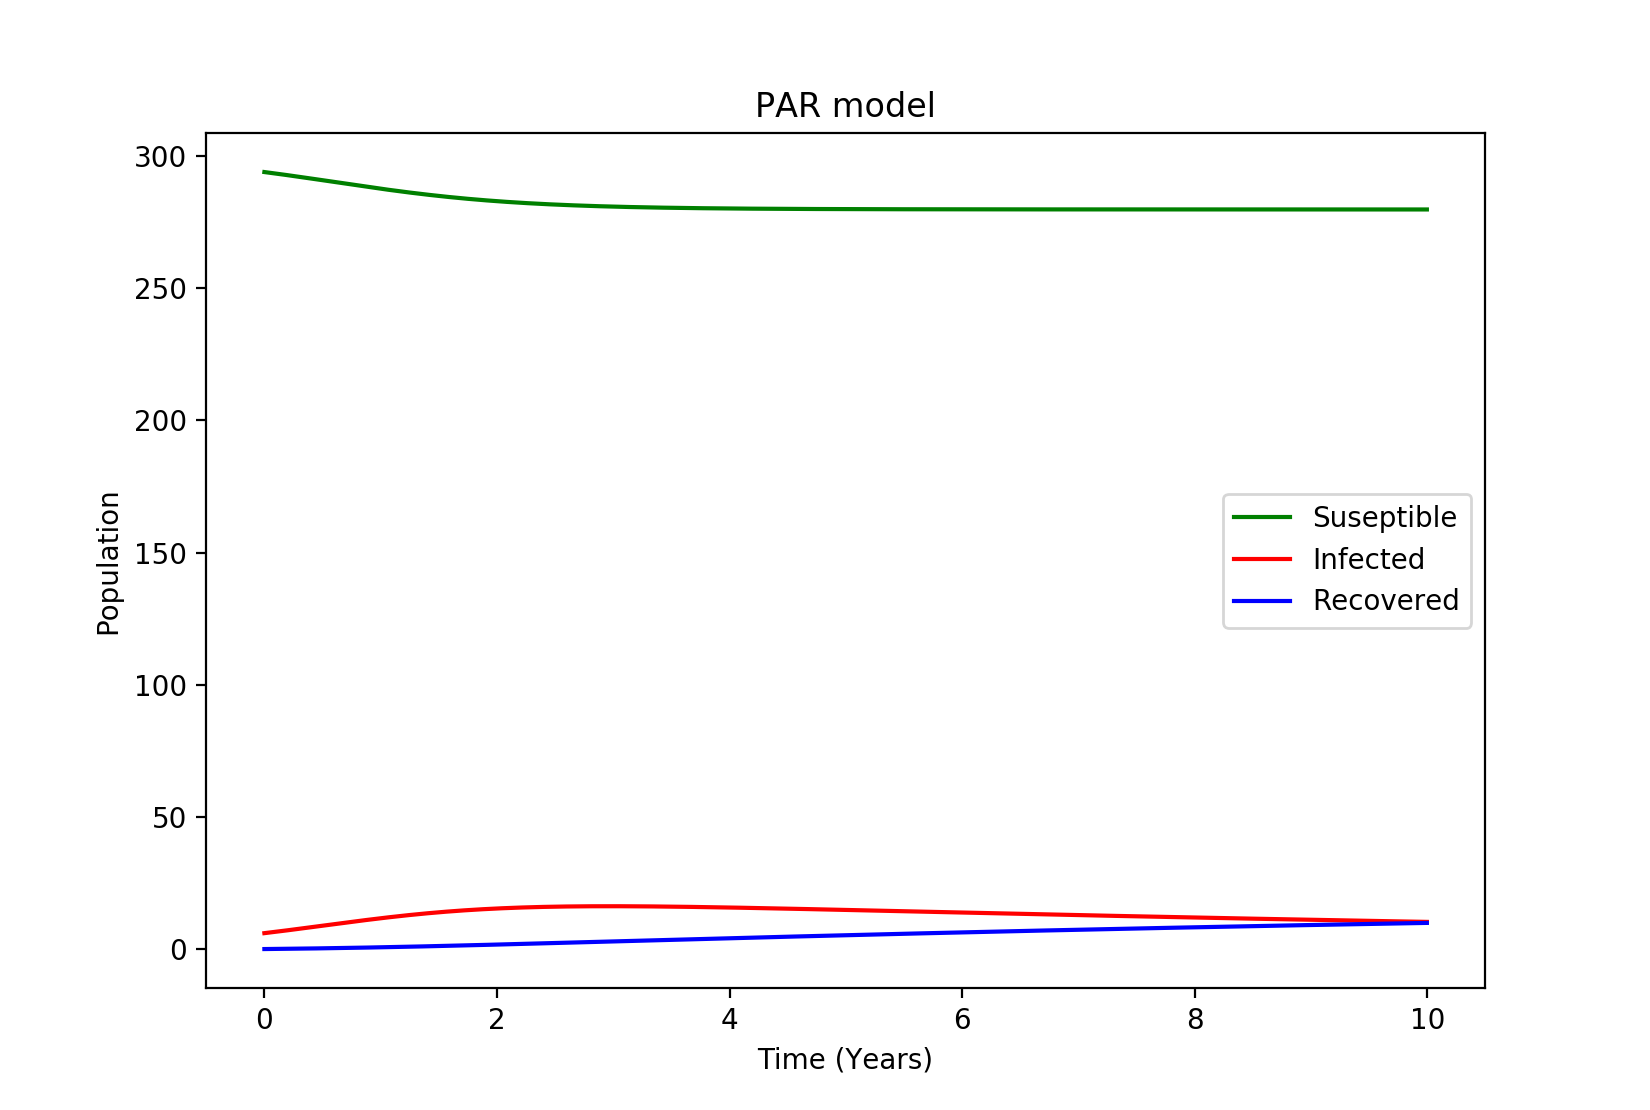
\includegraphics[width=.8\linewidth]{opium}
  \caption{PAR model for opium}
  \label{fig:opium}
\end{figure}

\begin{figure}[H]
  \centering
  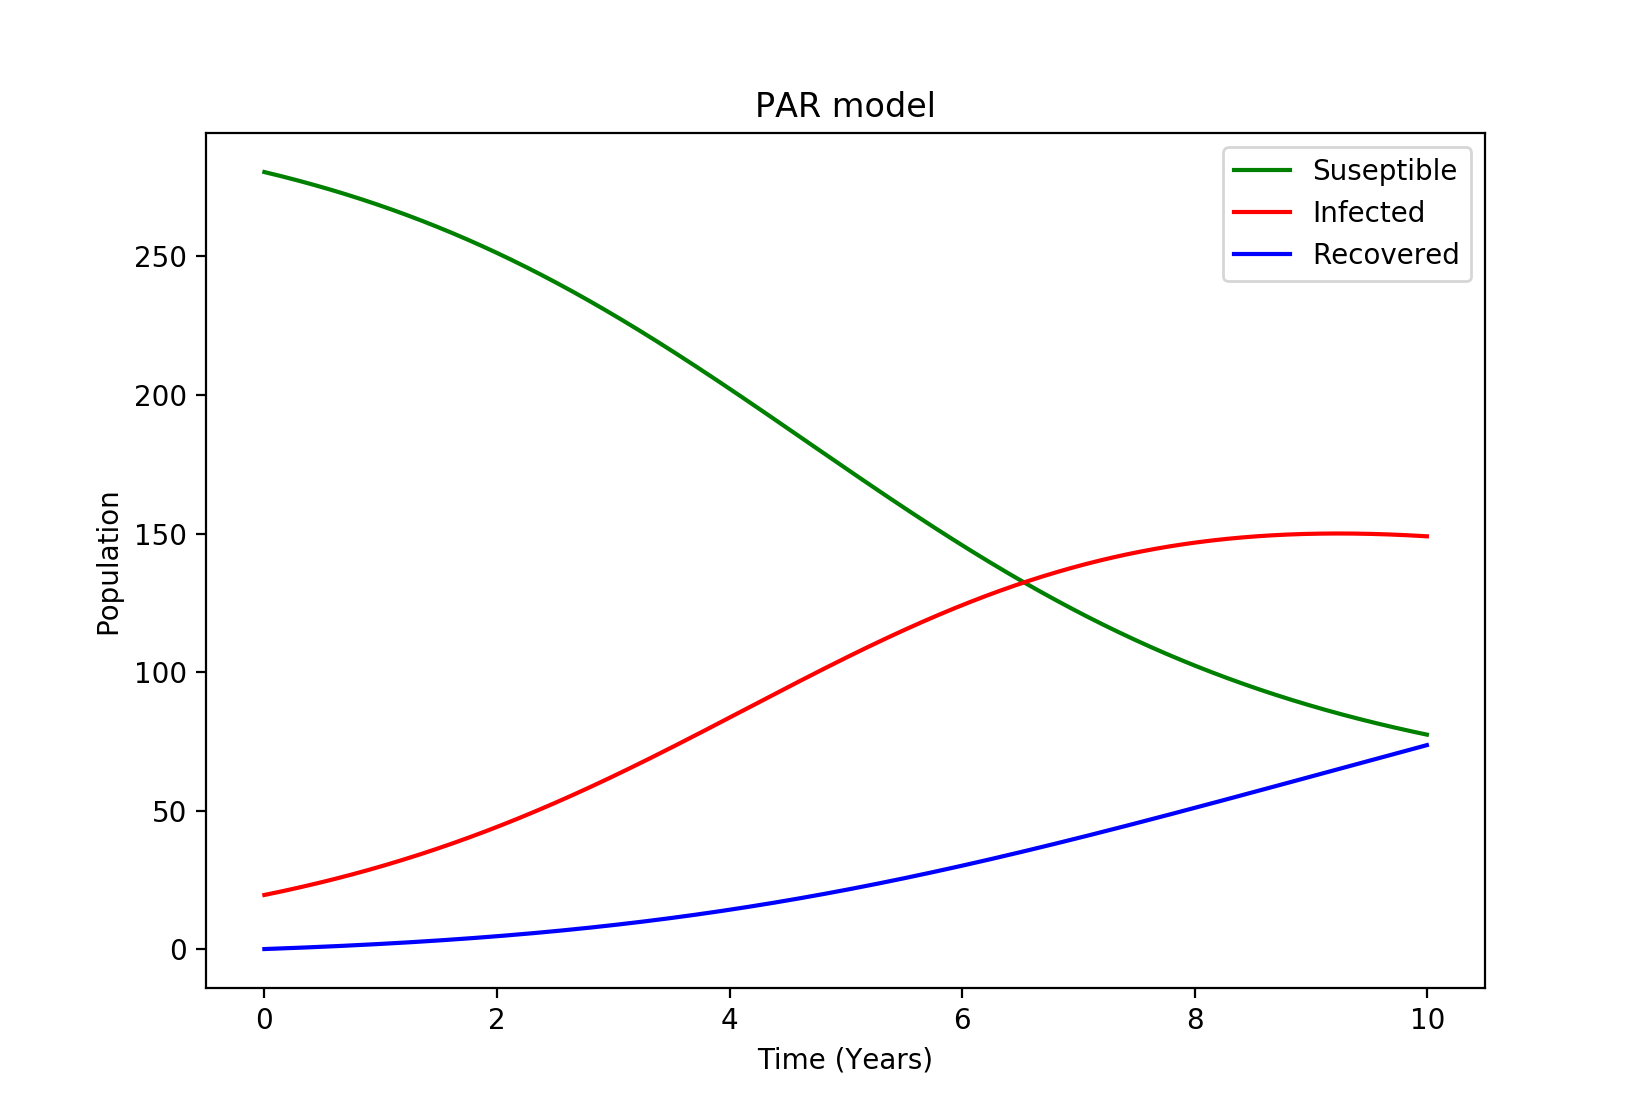
\includegraphics[width=.8\linewidth]{marijuana}
  \caption{PAR model for marijuana}
  \label{fig:marijuana}
\end{figure}

\begin{figure}[H]
  \centering
  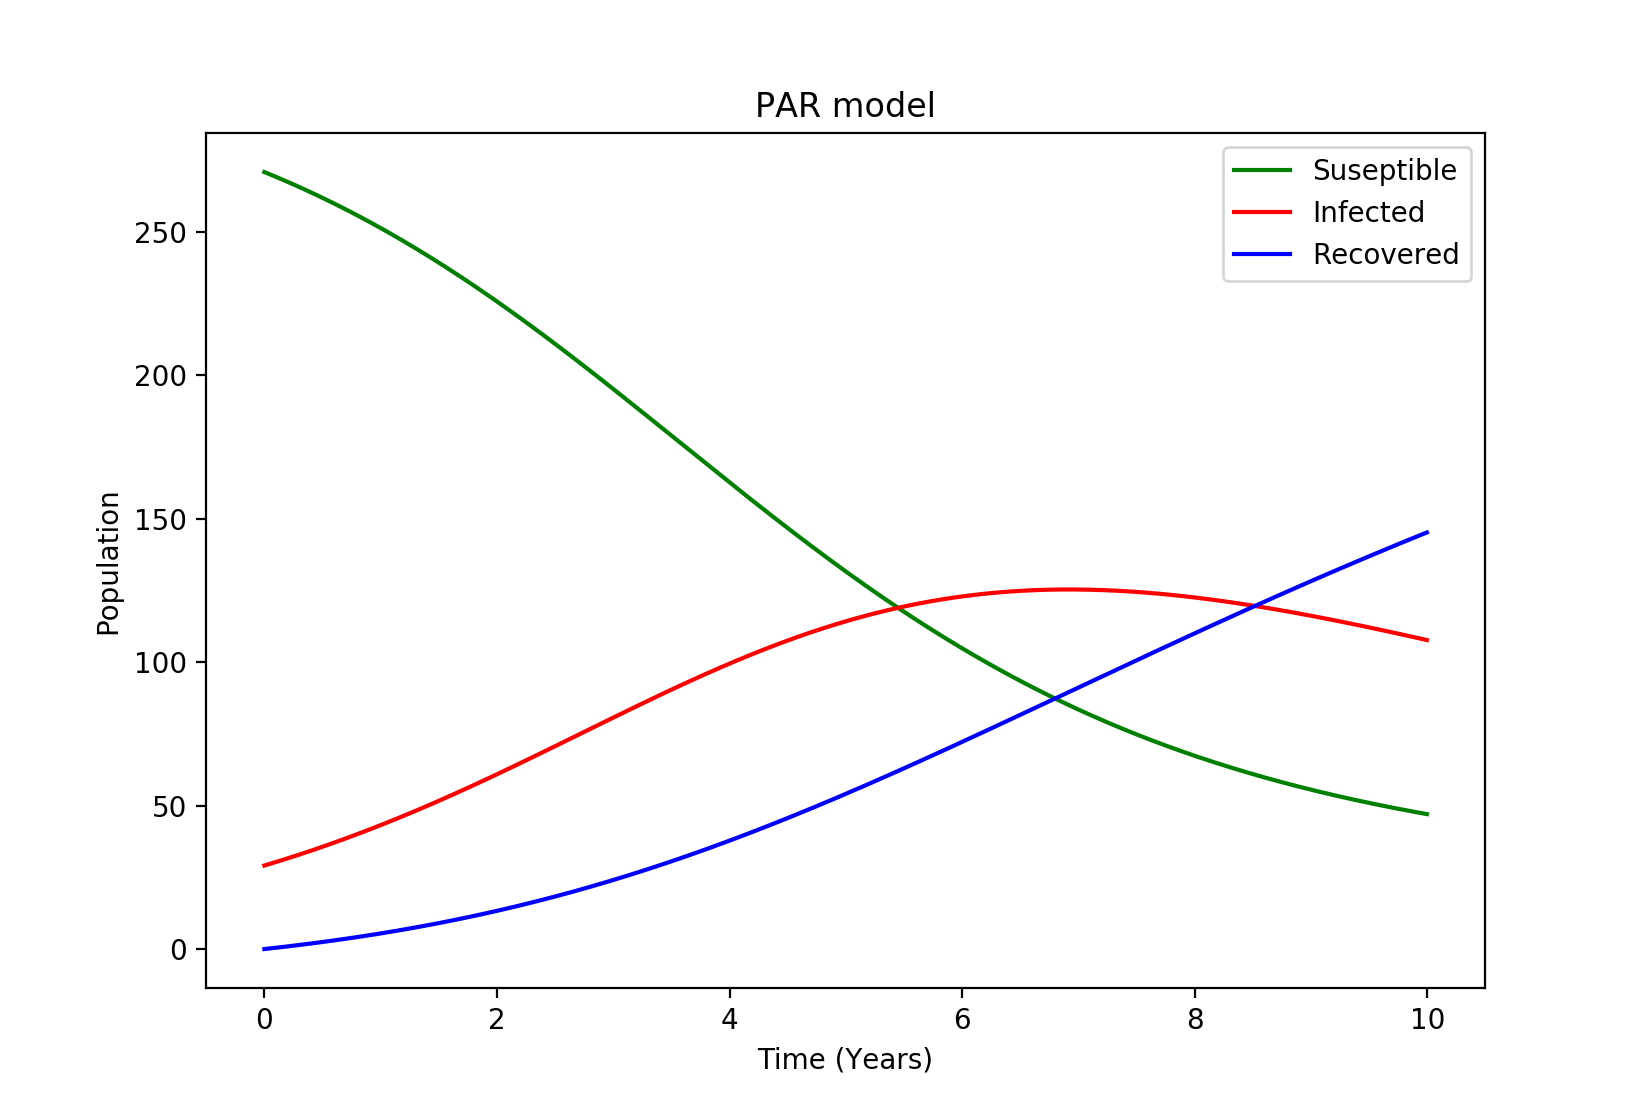
\includegraphics[width=.8\linewidth]{alcohol}
  \caption{PAR model for alcohol}
  \label{fig:alcohol}
\end{figure}

\begin{figure}[H]
  \centering
  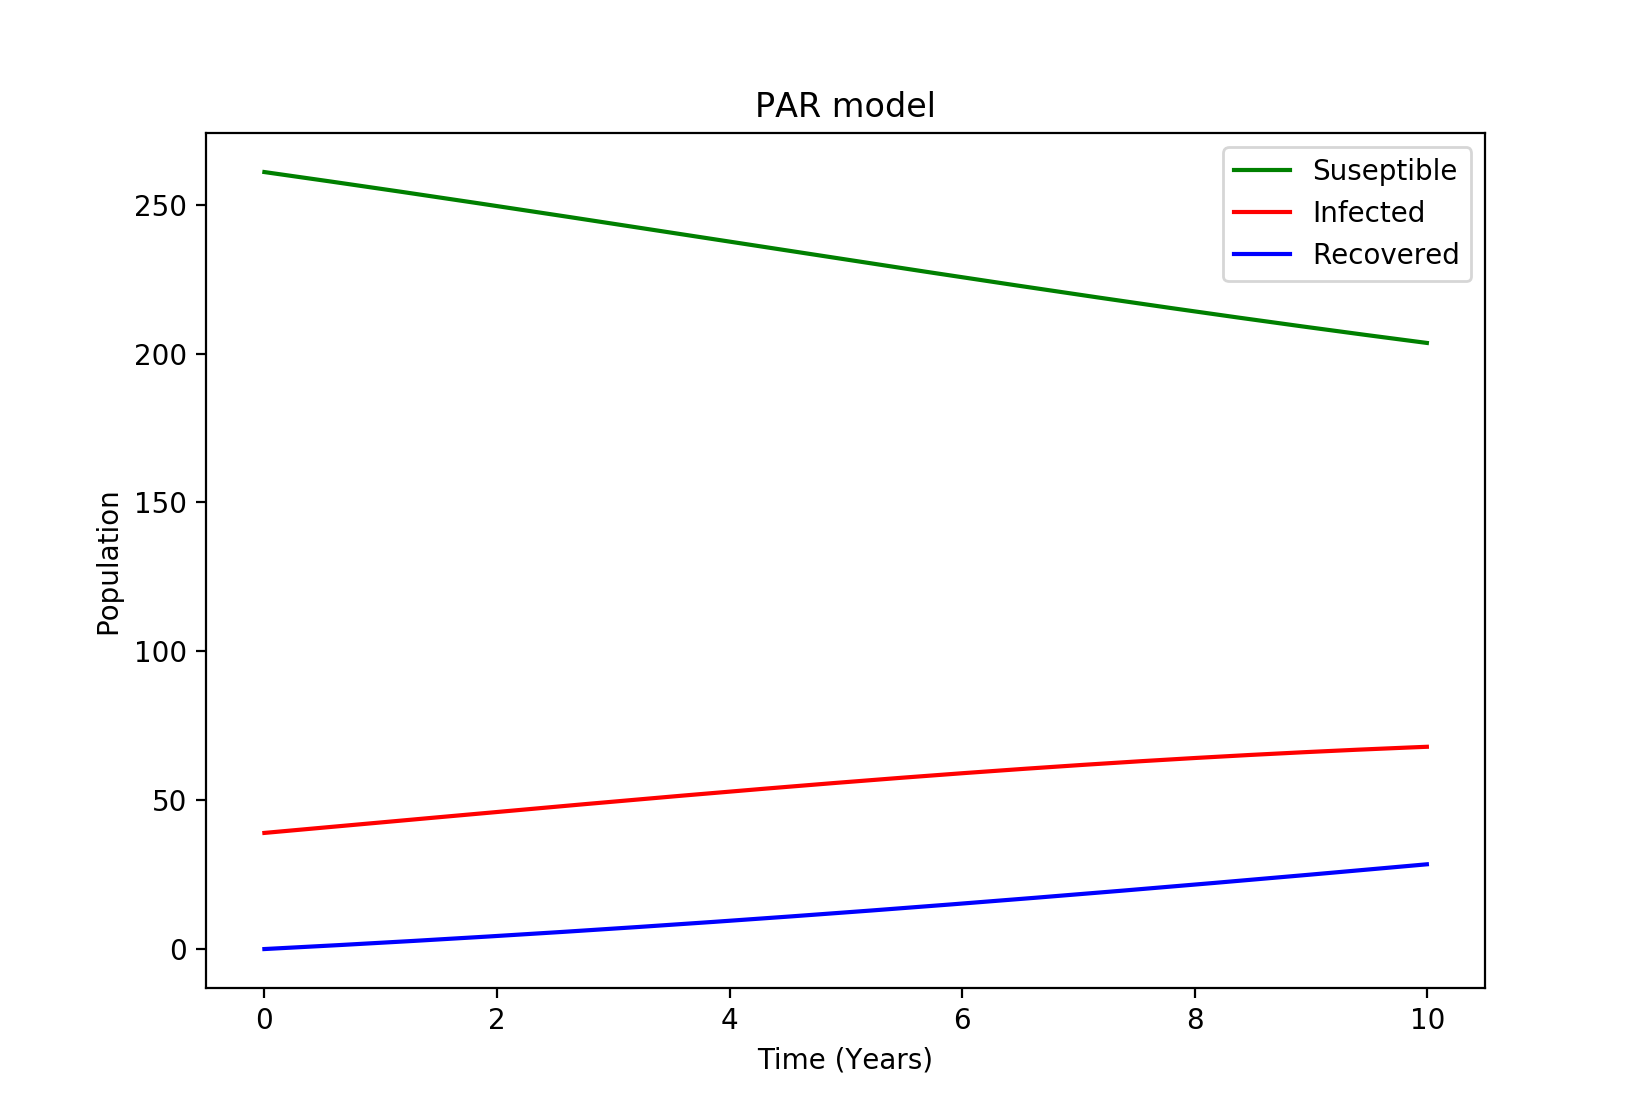
\includegraphics[width=.8\linewidth]{vape}
  \caption{PAR model for vaping}
  \label{fig:vape}
\end{figure}

\subsection{Strengths and Weaknesses}
\paragraph{Strengths}
\begin{itemize}
\item Usability: Our model is able to be extrapolated to multiple situations because it is based on being fine tuned by preexisting data. Therefore, if data already exists, once they are used to tune to model, it would theoretically work for any length of time for the given scenario.
\end{itemize}

\paragraph{Weaknesses}
\begin{itemize}
\item Interaction of Variables: Out Model uses multiple equations with variables used between them. Given a change in a single variable it is difficult to estimate the change in graphs. There is also unexpected interacts between different variables. It is not very intuitive
\item Similar to Previous Model: Due to the use of the SIR style model from the first section, any problems associated with that model also carry over to this model, along with many of its assumptions. 
\end{itemize}

\section{Ripples}
\subsection{Restatement of Problem}
We were asked to create a “robust” metric to describe the impact of using a given substance, and to account for both financial and non-financial factors, and then to rank the substances given in the above problem using our metric.

The term robust in this case is used to mean that the model is able to work in multiple scenarios, such as a wide variety of different drugs, in order to provide an accurate set of results in each case. When the constants are sufficiently tuned, the model can work given a range of possible starting configuration.


\subsection{Local Assumptions}
\begin{itemize}
  \item Cost of hospitalization is proportional to severity of hospitalization.
  \item The impact of death is taken into account under the subcategories of family toll and medical toll.
  \item For the rate of depression, we will be disregarding whether the mental illness set in before or after substance usage occurred; the relevant value will be perfect of users with mental illness of some sort.
  \item Sales tax is 6\% in all States.
\end{itemize}

\subsection{Variables}
The non-financial impacts of each drug can be roughly divided into three categories: a) Pain of family, b) medical toll on others, and c) personal health toll. Below is the identification of variables within these categories:

\begin{itemize}[label=]
  \item $P_{fam}$ = Pain of family
  \item $T_{ph}$ = Personal health toll
  \item $T_{med}$ = Medical toll on self and others
  \item $R_d$ = Rate of depression (constant throughout a year) or other mental illness as a percent
  \item $R_H$ = Rate of hospitalization as a percent
  \item $C_H$ = Estimated hospital cost (in tens of thousands)
  \item $n_{fam}$ = Average number of family members
  \item $S$ = Coefficient of severity for each drug (a number 1-10, used in association with $n_{fam}$)\footnote{This value will be assigned by us based on our research and overall impression of each substance}
  \item $I_{nf}$ = Total non-financial impact
\end{itemize}

\subsection{Solution and Results}

\begin{singlespace}
\begin{equation}
P_{fam} = S n_{fam}
\end{equation}
\begin{equation}
T_{ph} = \frac{Rd}{100} 20
\end{equation}
\begin{equation}
T_{med} = \frac{Rh}{100} C_H
\end{equation}

\begin{equation}
I_{nf} = P_{fam} + T_{ph} + T_{med}
\end{equation}
\end{singlespace}

The equation contains three sub-equations that are calculated separately and added together. These operations were used because the sub-equations (family pain, personal health toll, and medical toll) are all fairly separate conceptually and can have vastly different values independently of each other. A multiplier of 20 accompanies the personal health toll, $T_{ph}$, to normalize the value so it is not too insignificant or too overpowering over the other values.

\begin{figure}[H]
  \centering
  \csvautotabular{rippleVals.csv}
  \caption{Researched Values of Variables}
  The rate of hospitalization by nicotine is so small that it has negligible effect.
  Values collected from: \citep{noauthor_alcoholism_nodate}\citep{noauthor_risky_2017}\citep{cdctobaccofree_tobacco_2019}\citep{noauthor_depression_nodate}\citep{stahre_alcohol-related_2010}\citep{zhu_trends_2016}\citep{noauthor_opioid_nodate}\citep{noauthor_publications_nodate}\citep{pacula_incremental_2008}\citep{noauthor_what_2018}
\end{figure}

\begin{enumerate}
  \item Opioids: $I_{nf (opioids)}$ = (8.5(2.6)) + (20(.48)) + (6(25)) = 181.70
  \item Alcohol: $I_{nf (alcohol)}$ = (4(2.6)) + (20(0.60)) + (6(0.18)) =  23.48
  \item Nicotine: $I_{nf (nicotine)}$ = (2(2.6)) + (20(.32)) + (0) = 11.6
  \item Marijuana: $I_{nf (marijuana)}$ = (2(2.6)) + (20(.232)) + (0.226(0.0865)) = 9.86
\end{enumerate}

These rankings show that the drugs in order of qualitative effects from least to greatest are marijuana, nicotine, alcohol, and finally opioids. The non-financial impact for opioid usage is significantly larger than that of the other three substances, most likely due to the higher rate of hospitalization. The differences between non-financial impacts for alcohol, marijuana, and nicotine are all marginal, implying that in terms of the less easily quantifiable impacts, opioid usage is notable more damaging.

\begin{small}
\begin{singlespace}
\begin{equation}
\frac{dC}{dT} = -(C_j * P_j * A) - (C_m * P_m * A) - (1*T)(C_d * A)
\end{equation}
\begin{itemize}[label=]
\item $C_m$ = Medical Cost
\item $P_m$ = Percent with medical issues
\item $C_j$ = Jail Cost (\$40000)
\item $P_j$ = Percent in jail
\item $C_d$ = Cost of drugs
\item $T$ = Taxes (0.06)
\end{itemize}
\end{singlespace}
\end{small}

In estimating the financial cost of different forms of drug abuse, we figured out the average cost of jail per year per inmate which we estimated for \$40,000. We took into account the cost of the drugs and the affective income lost in this exchange when it comes to taxes and GDP/capita. For the different drugs we found different costs and rates of incarceration. To calculate the daily national cost we used the iterative calculations for the PAR model and then use the number of addicted people and the drug used to accumulate the cost of 10 years.

\paragraph{Costs per Drug}

The cost of addiction for an individual drug accumulated over 10 years.
\begin{enumerate}
\item Opioids cost over 10 years: \$1,784,529,013,157.3123
\item Weed cost over 10 years: \$856,641,880,044
\item Nicotine cost over 10 y: \$3,794,131,197,805
\item Alcoholism cost over 10 years: \$393,894,389,640
\end{enumerate}

\subsection{Strengths and Weaknesses}
\paragraph{Strengths}
\begin{itemize}
\item Variety of Variables: The wide array of variables that factor into this model allow it to be used to analyze many effects that are not usually quantified. The wide array of variables also makes the final value $I_{nf}$ more reliable, as no single variable holds too much power in the calculation.
\item Statistically Accurate: The vast majority of numerical figures used in the calculations are statistically valid and obtained from reliable sources, increasing their validity.
\end{itemize}

\paragraph{Weaknesses}
\begin{itemize}
\item Variables Subject to Change: The coefficient of severity, while not gathered arbitrarily, is based on the consensus of the group and is less ground in facts and statistics than the other quantities. The cost of incarceration varies based on the state of the person being admitted into the hospital.
\item Quantifying the Qualitative: For this section we had to take fundamentally qualitative data and compare them. In order to do that, we had to quantify this data and introduce arbitrary choices.
\end{itemize}

% \citep{national_academies_of_sciences_trends_2017}

\newpage
\printbibliography
% \bibliographystyle{IEEEtran}
\newpage

\appendix
\listoffigures
\listoftables

\section{Listings}
\subsection{SIR Model}
\lstinputlisting[language=Python, label={lst:surfaceCode}]{M3Code/model.py}
\subsection{Smoking Model}
\lstinputlisting[language=Python, label={lst:surfaceCode}]{M3Code/smoke.py}


\end{document}